\documentclass[11pt]{article}

\usepackage[letterpaper, margin=1in]{geometry}

\usepackage[spanish]{babel}
\usepackage[utf8]{inputenc}
\usepackage{multirow}
\usepackage{tabularx}
\usepackage{longtable}

\usepackage{listings}% Escribir código de programación



%Figuras
\usepackage{graphicx, subfigure}
\usepackage[]{tikz}
\usepackage{pbox}

%Matemática
\usepackage{amsmath}
\usepackage{amssymb}

%Símbolos mate extra (alfabetos, etc.)
\usepackage{mathrsfs}


%Algoritmos
\usepackage{float}
\usepackage{algorithm}
\usepackage{algorithmicx}
\usepackage{algpseudocode}
\usepackage{listings}


\usepackage{color}
\usepackage{hyperref}

\usepackage{mdframed}
\usepackage{tcolorbox}
\usepackage{multicol}
\usepackage{booktabs}
\usepackage{tabulary}
\definecolor{darkblue}{rgb}{0 , 0.054 , 0.196}



\title{Reporte de laboratorio 5}
\author{Laura Rincón Riveros - B55863\\Esteban Vargas Vargas - B16998\\ Grupo 3}

\begin{document}

\maketitle
\hrule
\hrule
\tableofcontents
\hspace{5mm}
\hrule
\hrule

%%%%%%%%%%%%%%%%%%%%%%%%%%%%%%%%%%%%
\section{Introducción}
%%%%%%%%%%%%%%%%%%%%%%%%%%%%%%%%%%%%

En el presente laboratorio se desarrolló un algotitmo que simula un casino, con el fin de implementar las colas y pilas; como se muestra a continuación:


\newpage
%%%%%%%%%%%%%%%%%%%%%%%%%%%%%%%%%%%%
\section{Desarrollo}
%%%%%%%%%%%%%%%%%%%%%%%%%%%%%%%%%%%%

%%%%%%%%%%%%%%%%%%%%%%
\subsection{Clase Lista}
%%%%%%%%%%%%%%%%%%%%%%

Se creó una clase emplantillada llamada Lista, en la cuál se definieron las funciones virtuales puras: agregar, eliminar e imprimir. Esta clase emplantillada puede recibir ListaConArreglo o ListaConPunteros, esta se presenta a continuación: 

\lstset {language=C}
\begin{lstlisting}


#ifndef LISTA_H
#define LISTA_H

template <typename T>
class Lista{ //lista de ints
public:
    Lista(){};
    Lista(const Lista& orig){};
    virtual ~Lista(){};

    virtual void agregar(T e) = 0;
    virtual void eliminar() = 0;
    virtual void eliminar_u()=0;
    virtual void imprimir() = 0;
private:

};

#endif /* LISTA_H */

\end{lstlisting}



\newpage
%%%%%%%%%%%%%%%%%%%%%%
\subsubsection{Clase ListaConArreglo}
%%%%%%%%%%%%%%%%%%%%%%

La clase ListaConArreglo hereda de Lista, también es una clase emplantillada. Esta clase implementa un lista con arreglos dinámicos, capaz de agregar y eliminar elementos del arreglo. 

Esta cuenta con los atributos: 
\begin{itemize}
\item \textit{int} tam : tamaño del arreglo.
\item \textit{int} ultimo
\item  data (type\_data$*$) = puntero a los elementos del arreglo.
\end{itemize}
Dado que Lista posee métodos virtuales puros, ListaConArreglo implementa los mismos de la siguiente manera:

\lstset {language=C}
\begin{lstlisting}

#ifndef LISTACONARREGLO_H
#define LISTACONARREGLO_H

#include <fstream>
#include <iostream>
#include <string>
#include <stdlib.h>
#include "Lista.h"

template<typename T>
class ListaConArreglo : public Lista<T> {
public:
    
    int tam;
    int ultimo;
    T* data; //almacenar los elementos
    
ListaConArreglo() {
    data = NULL;
    tam = 0;
    ultimo = -1;
}

ListaConArreglo(const ListaConArreglo& orig) {
}

~ListaConArreglo() {
}

ListaConArreglo(int N) {
    this->data = new T[N];
    tam = N;
    ultimo = tam - 1;
}

void agregar(T e) {
    if (data == 0) {
        data = new T[1];
        tam = 1;
        ultimo = 0;
        data[0] = e;
    } else {
        if (ultimo == tam - 1) {
            T* temp = new T[tam * 2];
            for (int i = 0; i < tam; i++) {
                temp[i] = data[i];
            }
            ultimo++;
            tam++;
            temp[ultimo] = e;
            delete data; 
            data = temp;
        } else {
            ultimo++;
            tam++;
            data[ultimo] = e;
        }
    }
}

void eliminarK(int k) {
    for (int i = k; i < tam - 1; i++) {
        data[i] = data[i + 1];
    }
    tam--;
    ultimo--;
}

virtual void eliminar() {
    eliminarK(0);
}

virtual void eliminar_u(){
    eliminarK(ultimo);
}

int buscar(T e) {
    for (int i = 0; i < tam; i++) {
        if (data[i] == e) {
            return i;
        }

    }
    return -1;
}

char siguienteK(int k) {
    if (k + 1 < tam) {
        return data[k + 1];
    } else {
        return -1;
    }
}

char anteriorK(int k) {
    if (k - 1 >= 0) {
        return data[k - 1];
    } else {
        return -1;
    }

}

T recuperar(int k) {
    return data[k];
}

void imprimir() {
    for (int i = 0; i < tam; i++) {
        std::cout << data[i] << "\t";
    }
    std::cout << std::endl;
}

};

#endif /* LISTACONARREGLO_H */


\end{lstlisting}


\begin{itemize}
\item agregar:
\item eliminar:
\item eliminarK:
\end{itemize}

Métodos adicionales:
\begin{itemize}
\item buscar:
\item siguienteK:
\item anteriorK:
\item recuperar:
\end{itemize}

\newpage 
%%%%%%%%%%%%%%%%%%%%%%
\subsubsection{Clase ListaConPunteros}
%%%%%%%%%%%%%%%%%%%%%%
La clase ListaConPuntero hereda de Lista. Esta clase implementa un lista con arreglos dinámicos, capaz de agregar y eliminar elementos del arreglo. También es una clase emplantillada.

Esta cuenta con los atributos: 
\begin{itemize}
\item \textit{$*$Celda$<T>*$}primera: cabeza de la lista.
\item \textit{$*$Celda$<T>*$}ultima: cola de la lista.
\item \textit{int} tam: tamaño de la lista. 
\end{itemize}

La clase Celda es una clase auxiliar, para que cada elemento de las lista posea: un valor, puntero a una celda siguiente y un puntero a una celda anterior. Lo anterior, para obtener un lista enlazada. 

Dado que Lista posee métodos virtuales puros, ListaConArreglo implementa los mismos de la siguiente manera:

\lstset {language=C}
\begin{lstlisting}



#ifndef LISTACONPUNTERO_H
#define LISTACONPUNTERO_H
#include "Lista.h"
#include "Celda.h"

#include <fstream>
#include <iostream>
#include <string>
#include <stdlib.h>

using namespace std;

template <typename T>
class ListaConPuntero : public Lista<T>{
public:
    
    Celda<T>* ultima;
    Celda<T>* primera;
    int tam;
    

ListaConPuntero(const ListaConPuntero& orig) {
}

~ListaConPuntero() {
    Celda<T>* ultima=NULL;
    Celda<T>* primera=NULL;
    tam = 0;
}


ListaConPuntero(int N) {
    Celda<T>* ultima=NULL;
    Celda<T>* primera=NULL;
    
    tam = N;

}

void agregar(T e) { //Se agrega al final
    Celda<T>* temp;
    if(this->primera==NULL){ //si es el primer elemento ingresado:
        Celda<T>* Casilla0 = new Celda<T>(e);
        this->primera =  Casilla0; //el unico elemento de la lista es la cabeza
        this->ultima= Casilla0; // y es la cola tambien
    }
    else{  // si hay mas elementos, se agrega al final
        
        Celda<T>* CasillaNueva= new Celda<T>(e);	
			
        Celda<T>* temp= ultima;		
		
        while (temp->siguiete!=NULL) {
            temp= temp->siguiete;
        }
        
        temp->siguiete= CasillaNueva;
    }
    tam++;
         
}

virtual void eliminar() { //se elimina el ultimo elemento
    if(tam>0){
        Celda<T>* temp_penultima;		
        Celda<T>* temp= primera;		

        while (temp->siguiete!=NULL) {
            temp_penultima= temp;
                temp= temp->siguiete;
        }
        ///////////////////////////////////////////////////
        temp_penultima->siguiete= NULL;
        delete temp;
        tam--;
    }
}   

T ultimo_elemento(){
    return this->ultima->valor;
}


void imprimir() { //recorre segun los punteros de la siguiente casilla, hasta llegar a un NULL.
   Celda<T>* Casilla= this->primera;
   int cont= 0;
   while(Casilla!=NULL && cont<=tam-1){
       cont++;
       cout << Casilla->valor << "\t";
       
       if(Casilla->siguiete!=NULL){
            Casilla = Casilla->siguiete;
       }
   }
   std::cout << std::endl;
}
    
   

};

#endif /* LISTACONPUNTERO_H */

\end{lstlisting}


\begin{itemize}
\item agregar: esta función agrega el elemento de parámatro al final de la fina, es decir, modifica el puntero de la última celda para que apunte al valor ingresado.
\item eliminar: al ejecutar esta función se elimina el primer elemento de la cola, es decir, la cabeza de la lista pasa a ser la siguiente celda.
\item imprimir: imprime el valor del primer apuntero hasta lo
\end{itemize}



%%%%%%%%%%%%%%%%%%%%%%
\newpage 
\subsection{Clase Portero}
Esta clase se encarga de la admisión de los clientes al casino. Esto se hace mediante una cola de prioridad, la cual según el estatus economico de los mismos los acomoda en un orden. La proporción de la cola de prioridad es 2:1:0,5 para los ejecutivos, trabajadores y desempleados; respectivamente. 

Para poder realizar esta tarea, se elaboró la clase con los atributos siguientes:
\begin{itemize}
\item \textit{int} cantidad$\_$clientes: es la cantidad de personas se encuentran en la cola para entrar al casino.
\item \textit{int} ejecutivos: número de clientes que cuentan con mayor poder adquisitivo y por ende tienen prioridad 2.
\item \textit{int} trabajadores: número de clientes que cuentan con normal poder adquisitivo y por ende tienen prioridad 1.
\item \textit{int} desempleados: número de clientes que cuentan con bajo poder adquisitivo y por ende tienen prioridad 0,5.

Además de estos atributos también se crearon salas de espera para los ejecutivos(sala$\_$espera$\_$E), trabajadores(sala$\_$espera$\_$T) y desempleados(sala$\_$espera$\_$D); para después obtener la cola final, la cual también es un atributo (sala$\_$final).
\end{itemize}


Las funciones pertenecientes a esta clase son:
\begin{itemize}
\item \textit{void} \textbf{categorizar}(): realiza la función de agarrar la entrada del programa, la cual se introduce por consola, y ordenarla en la cola de prioridad ya mencionada. 
\item \textit{void} \textbf{eliminardeCola}():como su nombre lo indica, elimina a algún cliente de la cola de prioridad.
\item \textit{char} tipo: retorna el tipo de algún jugador.
\end{itemize}
%%%%%%%%%%%%%%%%%%
\subsection{Clase jugador}
El objeto Jugador tiene 3 atributos de suma importancia:
\begin{itemize}
\item \textit{int} acumulado: es el puntaje que lleva el jugador, dadas las cartas que tiene en su mano en algún momento dado.
\item \textit{char} id:es la identificación del estatus económico de cada jugador. Puede ser 'E' para ejecutivo, 'T' para trabajador y 'D' para desempleado. 
\item \textit{int} estado: Puede tomar tres valores: 0, 1 y 2. Cuando el estado es 0 significa que el jugador está inactivo y se encuentra en fila. Si el estado es 1 entonces se encuentra en la mesa jugando. En el caso de que el estado sea igual a 2 entonces el jugador perdió. 
\end{itemize}

La única función con la que cuenta esta clase es \textbf{perder()}. Esta se llama cuando algún jugador tiene un acumulado mayor a 21. Le resetea su acumulado y lo expulsa de la mesa. 

\subsection{Clase Mesa}
La clase mesa implementa la lógica del juego. Para ello necesita de las clases ya mencionadas. Ella misma cuenta con atributos propios:
\begin{itemize}
\item \textit{int} cantidad$\_$jugadores
\item \textit{Jugador*} jugador1  
\item \textit{Jugador*} jugador2
\item \textit{Jugador*} jugador3
\end{itemize}

Asimismo cuenta con las siguientes funciones:
\begin{itemize}
\item \textit{void} \textbf{jugar}: Inicia la partida. Recibe como parámetros las 3 mesas del casino.
\item \textit{void} \textbf{imprimir$\_$estado}(); imprime el estado de cada mesa antes y después de una partida. 
\end{itemize}







\subsubsection{Clase Mazo}
El mazo es una estructura de datos conocida como "pila". Esta se parece a una lista, sin embargo tiene la característica de que le último elemento que entra es el primero en salir. Para este caso, se elaboró una pila de objetos carta.

Estas cartas se hicieron como atributos de la clase. Se introdujeron 52 de estas, como en un mazo de cartas convencional. Además de esto se hizo ya propiamente el atributo relevante a esta clase, que es la baraja; un puntero de tipo Carta.  

Como funciones, la clase cuenta con las siguientes:
\begin{itemize}
\item \textit{void} \textbf{barajar}(): la cual toma el arreglo de cartas, o baraja, y lo revuelve.
\item \textit{void} \textbf{print}(): imprime los datos de las 52 cartas de la baraja. 
\end{itemize}

\subsubsection{Clase Carta}
La clase Carta es un objeto que tiene los siguientes atributos:
\begin{itemize}
\item \textit{int} Valor: es el valor numérico que tiene cada carta, el cual se acumula cuando la recibe cada jugador. Para los números del 2 al 10 es su mismo valor numérico; para el \textit{as} es 11, la \textit{jota,quina y ka} son 10. 
\item \textit{String} Nombre: es el identificador de cada carta.
\item \textit{String} Palo: puede ser espada, corazón, trébol o diamante. 
\end{itemize}

Únicamente cuenta con un método \textit{void} llamado \textbf{imprimir}. El cual imprime en consola los datos de la carta, osea su valor, nombre y palo. 

\newpage
%%%%%%%%%%%%%%%%%%%%%%
\subsection{Main}
En el main se crearon los jugadores, según la cola de prioridad, se crearon las mesas y se llamó a la función de jugar. Se implementó el código de tal forma que se jugaran manos en cada mesa hasta que ya la cola de espera estuviera vacía. A continuación se muestra el código. 

\begin{lstlisting}


#include <cstdlib>
#include"Carta.h"
#include "Mazo.h"
#include "ListaConArreglo.h"
#include "ListaConPuntero.h"
#include "Portero.h"
#include "Jugador.h"
#include "Mesa.h"
int main(int argc, char** argv) {
    
    int i=0;
    int len=0;
    int contEjecutivo=0;
    int contTrabajador=0;
    int contDesempleado=0;
    
    ///Para contar el numero de clientes y cuantos ejecutivos, trabajadores y desempleados hay
    while(argv[1][i]!='\0'){
        if(argv[1][i]=='e'||argv[1][i]=='E'){
            contEjecutivo++;
        }
        if(argv[1][i]=='t'||argv[1][i]=='T'){
            contTrabajador++;
        }
        if(argv[1][i]=='d'||argv[1][i]=='D'){
            contDesempleado++;
        }
        len++;
        i++;
    }
    cout<< "Largo fila: " << len << endl;
    cout<< "Ejecutivos: " << contEjecutivo<<endl;
    cout<< "Trabajadores: " << contTrabajador<<endl;
    cout<< "Desempleados: " << contDesempleado<<endl;
    
    ///Creacion mazos
    Mazo mazo1= Mazo();
    Mazo mazo2= Mazo();
    Mazo mazo3= Mazo();
    
    
    ///Creacion portero
    Portero P = Portero(argv[1],len,contEjecutivo,contTrabajador,contDesempleado);
    P.categorizar();
    
    ///Creacion de un arreglo de objetos tipo Jugador
    Jugador* jugadores[len];
    int a=0;
    for(int i=0; i<len;i++){
        jugadores[i]= new Jugador(P.sala_final.recuperar(i));
        a++;
    }
    int* esperando_turno=new int[1];
    esperando_turno[0]=a-9;
    int b=a-9;
    
    ///Creacion mesas
    Mesa casino= Mesa();
    
    Mesa* mesa1 = new Mesa(jugadores[0],jugadores[1],jugadores[2],mazo1);
    Mesa* mesa2 = new Mesa(jugadores[3],jugadores[4],jugadores[5],mazo2);
    Mesa* mesa3 = new Mesa(jugadores[6],jugadores[7],jugadores[8],mazo3);
    
    casino.jugar(P,mesa1,mesa2,mesa3);      

    
    //PARA JUGAR VARIAS MANOS, SE VERIFICA CUALES JUGADORES PERDIERON Y SE REEMPLAZAN POR LOS QUE ESTAN ESPERANDO
    while(esperando_turno[0]>0){
        //Verificacion mesa 2

        if(mesa1->jugador1->estado==2){
            Mesa* mesa1=new Mesa(jugadores[b],jugadores[1],jugadores[2],mazo1);
            esperando_turno[0]=esperando_turno[0]-1;
            b++;
        }
        if(mesa1->jugador2->estado==2){
            Mesa* mesa1=new Mesa(jugadores[0],jugadores[b],jugadores[2],mazo1);
            esperando_turno[0]=esperando_turno[0]-1;
            b++;
        }
        if(mesa1->jugador3->estado==2){
            Mesa* mesa1=new Mesa(jugadores[0],jugadores[1],jugadores[b],mazo1);
            esperando_turno[0]=esperando_turno[0]-1;
            b++;
        }
        //Verificacion mesa 2
        if(mesa2->jugador1->estado==2){
            Mesa* mesa2=new Mesa(jugadores[b],jugadores[1],jugadores[2],mazo1);
            esperando_turno[0]=esperando_turno[0]-1;
            b++;
        }
        if(mesa2->jugador2->estado==2){
            Mesa* mesa2=new Mesa(jugadores[0],jugadores[b],jugadores[2],mazo1);
            esperando_turno[0]=esperando_turno[0]-1;
            b++;
        }
        if(mesa2->jugador3->estado==2){
            Mesa* mesa2=new Mesa(jugadores[0],jugadores[1],jugadores[b],mazo1);
            esperando_turno[0]=esperando_turno[0]-1;
            b++;
        }        
        
        //Verificacion mesa 3
        if(mesa3->jugador1->estado==2){
            Mesa* mesa3=new Mesa(jugadores[b],jugadores[1],jugadores[2],mazo1);
            esperando_turno[0]=esperando_turno[0]-1;
            b++;
        }
        if(mesa3->jugador2->estado==2){
            Mesa* mesa3=new Mesa(jugadores[0],jugadores[b],jugadores[2],mazo1);
            esperando_turno[0]=esperando_turno[0]-1;
            b++;
        }
        if(mesa3->jugador3->estado==2){
            Mesa* mesa3=new Mesa(jugadores[0],jugadores[1],jugadores[b],mazo1);
            esperando_turno[0]=esperando_turno[0]-1;
            b++;
        }
        casino.jugar(P,mesa1,mesa2,mesa3);
    }
    return 0;
}
\end{lstlisting}
%%%%%%%%%%%%%%%%%%%%%%


\newpage
%%%%%%%%%%%%%%%%%%%%%%
\subsection{Diagramas}
%%%%%%%%%%%%%%%%%%%%%%
Para una mejor visualización de la composición de las clases se presenta a continuación el diagrama de colaboración para la clase Mesa, la cual utiliza objetos tipo mazo(este usa carta) y jugador.

\begin{figure}[htbp]
\centering
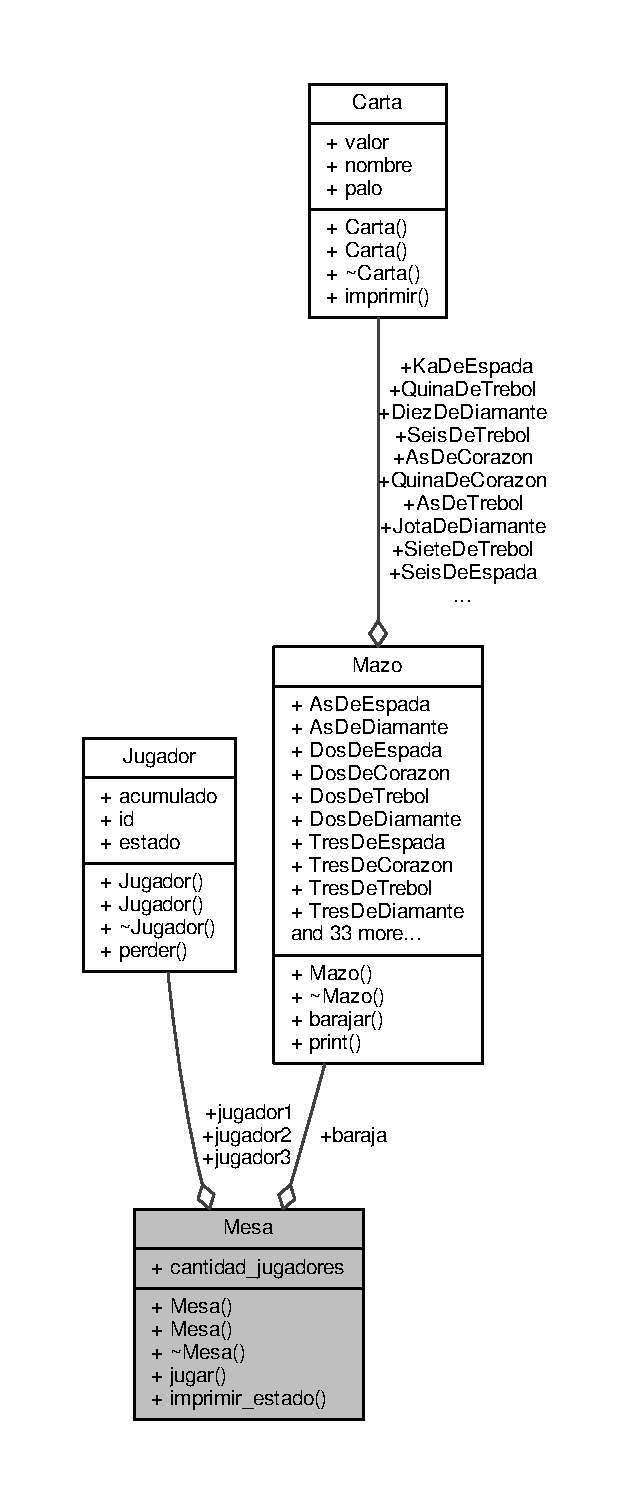
\includegraphics[width=0.55\textwidth]{img/class_mesa__coll__graph.pdf}
\caption{\label{fig:umlcalc} Diagrama colaboración clase Mesa}
\end{figure}



 
\newpage
%%%%%%%%%%%%%%%%%%%%%%%%%%%%%%%%
\section{Conclusiones}
%%%%%%%%%%%%%%%%%%%%%%%%%%%%%%%%
\begin{itemize}
\item Se emplantillaron listas para poder utilizarlas con distintos objetos.
\item Se implementó las reglas y funcionalidad del juego BlackJack.
\item Se implementó la cola de prioridad para organizar la cola de personas en el Casino.
\item No se pudo repartir varias manos en las mesas ya que se presentó un problema de enciclamiento que no se logró resolver.
\end{itemize}
\newpage
 
\section{Anexos}
\subsection{Carta.h}
\begin{lstlisting}
#ifndef CARTA_H
#define CARTA_H

#include <iostream>
using namespace std;
#include <string>

class Carta{
public:
    ///Constructores y destructores de Carta
	Carta();
	Carta(int valor, string nombre, string palo);
	virtual ~Carta();
    ///Atributos de Carta
	int valor;
	string nombre;
	string palo;
    ///Funciones de Carta
	void imprimir();

	
};


#endif /* CARTA_H */
\end{lstlisting}

\newpage
\subsection{Carta.cpp}
\begin{lstlisting}
#include "Carta.h"

Carta::Carta() {
}

Carta::Carta(int valor, string nombre, string palo){
	this->valor = valor;
	this->nombre = nombre;
	this->palo = palo;

}

Carta::~Carta(){
}

void Carta::imprimir(){
	cout<< "Nombre de la carta es: " << this->nombre <<endl;
	cout<< "Valor de la carta es: " << this->valor <<endl;
	cout<< "El palo de la carta es: " << this->palo <<endl;
//Los palos pueden ser: espada,corazon,diamante y trebol
}
\end{lstlisting}
\newpage

\subsection{Mazo.h}
\begin{lstlisting}
#ifndef MAZO_H
#define MAZO_H
#include "Carta.h"
#include <string>
#include "ListaConArreglo.h"
#include "ListaConPuntero.h"
#include <algorithm>


class Mazo{
public:
    ///Constructor de Mazo
	Mazo();
    ///Destructor de Mazo
	virtual ~Mazo();
    ///Atributos
        Carta AsDeEspada;
        Carta AsDeCorazon;
        Carta AsDeTrebol;
        Carta AsDeDiamante;

        Carta DosDeEspada;
        Carta DosDeCorazon;
        Carta DosDeTrebol;
        Carta DosDeDiamante;

        Carta TresDeEspada;
        Carta TresDeCorazon;
        Carta TresDeTrebol;
        Carta TresDeDiamante;

        Carta CuatroDeEspada;
        Carta CuatroDeCorazon;
        Carta CuatroDeTrebol;
        Carta CuatroDeDiamante;

        Carta CincoDeEspada;
        Carta CincoDeCorazon;
        Carta CincoDeTrebol;
        Carta CincoDeDiamante;

        Carta SeisDeEspada;
        Carta SeisDeCorazon;
        Carta SeisDeTrebol;
        Carta SeisDeDiamante;

        Carta SieteDeEspada;
        Carta SieteDeCorazon;
        Carta SieteDeTrebol;
        Carta SieteDeDiamante;

        Carta OchoDeEspada;
        Carta OchoDeCorazon;
        Carta OchoDeTrebol;
        Carta OchoDeDiamante;

        Carta NueveDeEspada;
        Carta NueveDeCorazon;
        Carta NueveDeTrebol;
        Carta NueveDeDiamante;

        Carta DiezDeEspada;
        Carta DiezDeCorazon;
        Carta DiezDeTrebol;
        Carta DiezDeDiamante;

        Carta JotaDeEspada;
        Carta JotaDeCorazon;
        Carta JotaDeTrebol;
        Carta JotaDeDiamante;

        Carta QuinaDeEspada;
        Carta QuinaDeCorazon;
        Carta QuinaDeTrebol;
        Carta QuinaDeDiamante;

        Carta KaDeEspada;
        Carta KaDeCorazon;
        Carta KaDeTrebol;
        Carta KaDeDiamante;
        
        Carta* baraja = new Carta[52];
        
        
    ///Funciones
        void barajar();
        void print();
};

#endif /* MAZO_H */
\end{lstlisting}
\newpage

\subsection{Mazo.cpp}
\begin{lstlisting}
#include "Mazo.h"

Mazo::Mazo(){
    this->AsDeEspada= Carta(11,"As de espada", "Espada");
    this->AsDeCorazon= Carta(11,"As de corazon", "Corazon");
    this->AsDeTrebol= Carta(11,"As de trebol", "Corazon");
    this->AsDeDiamante= Carta(11,"As de diamante", "Diamante");
    
    this->DosDeEspada= Carta(2,"Dos de espada", "Espada");
    this->DosDeCorazon= Carta(2,"Dos de corazon", "Corazon");
    this->DosDeTrebol= Carta(2,"Dos de trebol", "Corazon");
    this->DosDeDiamante= Carta(2,"Dos de diamante", "Diamante");

    this->TresDeEspada= Carta(3,"Tres de espada", "Espada");
    this->TresDeCorazon= Carta(3,"Tres de corazon", "Corazon");
    this->TresDeTrebol= Carta(3,"Tres de trebol", "Corazon");
    this->TresDeDiamante= Carta(3,"Tres de diamante", "Diamante");

    this->CuatroDeEspada= Carta(4,"Cuatro de espada", "Espada");
    this->CuatroDeCorazon= Carta(4,"Cuatro de corazon", "Corazon");
    this->CuatroDeTrebol= Carta(4,"Cuatro de trebol", "Corazon");
    this->CuatroDeDiamante= Carta(4,"Cuatro de diamante", "Diamante");

    this->CincoDeEspada= Carta(5,"Cinco de espada", "Espada");
    this->CincoDeCorazon= Carta(5,"Cinco de corazon", "Corazon");
    this->CincoDeTrebol= Carta(5,"Cinco de trebol", "Corazon");
    this->CincoDeDiamante= Carta(5,"Cinco de diamante", "Diamante");

    this->SeisDeEspada= Carta(6,"Seis de espada", "Espada");
    this->SeisDeCorazon= Carta(6,"Seis de corazon", "Corazon");
    this->SeisDeTrebol= Carta(6,"Seis de trebol", "Corazon");
    this->SeisDeDiamante= Carta(6,"Seis de diamante", "Diamante");

    this->SieteDeEspada= Carta(7,"Siete de espada", "Espada");
    this->SieteDeCorazon= Carta(7,"Siete de corazon", "Corazon");
    this->SieteDeTrebol= Carta(7,"Siete de trebol", "Corazon");
    this->SieteDeDiamante= Carta(7,"Siete de diamante", "Diamante");    

    this->OchoDeEspada= Carta(8,"Ocho de espada", "Espada");
    this->OchoDeCorazon= Carta(8,"Ocho de corazon", "Corazon");
    this->OchoDeTrebol= Carta(8,"Ocho de trebol", "Corazon");
    this->OchoDeDiamante= Carta(8,"Ocho de diamante", "Diamante");    

    this->NueveDeEspada= Carta(9,"Nueve de espada", "Espada");
    this->NueveDeCorazon= Carta(9,"Nueve de corazon", "Corazon");
    this->NueveDeTrebol= Carta(9,"Nueve de trebol", "Corazon");
    this->NueveDeDiamante= Carta(9,"Nueve de diamante", "Diamante");    

    this->DiezDeEspada= Carta(10,"Diez de espada", "Espada");
    this->DiezDeCorazon= Carta(10,"Diez de corazon", "Corazon");
    this->DiezDeTrebol= Carta(10,"Diez de trebol", "Corazon");
    this->DiezDeDiamante= Carta(10,"Diez de diamante", "Diamante");    

    this->JotaDeEspada= Carta(10,"Jota de espada", "Espada");
    this->JotaDeCorazon= Carta(10,"Jota de corazon", "Corazon");
    this->JotaDeTrebol= Carta(10,"Jota de trebol", "Corazon");
    this->JotaDeDiamante= Carta(10,"Jota de diamante", "Diamante");    

    this->QuinaDeEspada= Carta(10,"Quina de espada", "Espada");
    this->QuinaDeCorazon= Carta(10,"Quina de corazon", "Corazon");
    this->QuinaDeTrebol= Carta(10,"Quina de trebol", "Corazon");
    this->QuinaDeDiamante= Carta(10,"Quina de diamante", "Diamante");    

    this->KaDeEspada= Carta(10,"Ka de espada", "Espada");
    this->KaDeCorazon= Carta(10,"Ka de corazon", "Corazon");
    this->KaDeTrebol= Carta(10,"Ka de trebol", "Corazon");
    this->KaDeDiamante= Carta(10,"Ka de diamante", "Diamante");    
    
    //this->baraja = new ListaConArreglo();
    //this->baraja= {AsDeEspada};
    
    this->baraja[0]=AsDeEspada;
    this->baraja[1]=AsDeCorazon;
    this->baraja[2]=AsDeTrebol;
    this->baraja[3]=AsDeDiamante;
    
    this->baraja[4]=DosDeEspada;
    this->baraja[5]=DosDeCorazon;
    this->baraja[6]=DosDeTrebol;
    this->baraja[7]=DosDeDiamante;
    
    this->baraja[8]=TresDeEspada;
    this->baraja[9]=TresDeCorazon;
    this->baraja[10]=TresDeTrebol;
    this->baraja[11]=TresDeDiamante;
    
    this->baraja[12]=CuatroDeEspada;
    this->baraja[13]=CuatroDeCorazon;
    this->baraja[14]=CuatroDeTrebol;
    this->baraja[15]=CuatroDeDiamante;
    
    this->baraja[16]=CincoDeEspada;
    this->baraja[17]=CincoDeCorazon;
    this->baraja[18]=CincoDeTrebol;
    this->baraja[19]=CincoDeDiamante;
    
    this->baraja[20]=SeisDeEspada;
    this->baraja[21]=SeisDeCorazon;
    this->baraja[22]=SeisDeTrebol;
    this->baraja[23]=SeisDeDiamante;
    
    this->baraja[24]=SieteDeEspada;
    this->baraja[25]=SieteDeCorazon;
    this->baraja[26]=SieteDeTrebol;
    this->baraja[27]=SieteDeDiamante;
    
    this->baraja[28]=OchoDeEspada;
    this->baraja[29]=OchoDeCorazon;
    this->baraja[30]=OchoDeTrebol;
    this->baraja[31]=OchoDeDiamante;
    
    this->baraja[32]=NueveDeEspada;
    this->baraja[33]=NueveDeCorazon;
    this->baraja[34]=NueveDeTrebol;
    this->baraja[35]=NueveDeDiamante;
    
    this->baraja[36]=DiezDeEspada;
    this->baraja[37]=DiezDeCorazon;
    this->baraja[38]=DiezDeTrebol;
    this->baraja[39]=DiezDeDiamante;
    
    this->baraja[40]=JotaDeEspada;
    this->baraja[41]=JotaDeCorazon;
    this->baraja[42]=JotaDeTrebol;
    this->baraja[43]=JotaDeDiamante;
    
    this->baraja[44]=QuinaDeEspada;
    this->baraja[45]=QuinaDeCorazon;
    this->baraja[46]=QuinaDeTrebol;
    this->baraja[47]=QuinaDeDiamante;
    
    this->baraja[48]=KaDeEspada;
    this->baraja[49]=KaDeCorazon;
    this->baraja[50]=KaDeTrebol;
    this->baraja[51]=KaDeDiamante;
}

Mazo::~Mazo(){


}
void Mazo::barajar(){
    random_shuffle(&baraja[0],&baraja[52]);
}

void Mazo::print(){
    for(int i=0;i<52;i++){
        baraja[i].imprimir();
        cout<<endl;
    }

}
\end{lstlisting}
\newpage

\subsection{Jugador.h}
\begin{lstlisting}
#ifndef JUGADOR_H
#define JUGADOR_H

class Jugador{
    public: 
    ///Constructor vacio de Jugador
    Jugador();
    
    ///Constructor de Jugador
    Jugador(char id);
        
    ///Destructor de Portero
    virtual ~Jugador();
    
    ///Atributos del Potero
    int acumulado;
    char id;
    int estado;
    
    ///Funcion cuando un jugador pierde
    void perder();
};

#endif /* JUGADOR_H */
\end{lstlisting}
\newpage

\subsection{Jugador.cpp}
\begin{lstlisting}
#include "Jugador.h"
Jugador::Jugador(){

}

Jugador::Jugador(char id){
    this->id=id;
    this->acumulado=0;
    this->estado=0;
}

Jugador::~Jugador(){
    
}

void Jugador::perder(){
    this->estado=2;
}
\end{lstlisting}
\newpage

\subsection{Mesa.h}
\begin{lstlisting}
#ifndef MESA_H
#define MESA_H
#include "Mazo.h"
#include "Jugador.h"
#include "Portero.h" 

class Mesa{
    
public: 
    ///Constructor vacio de Mesa
    Mesa();
    
    ///Contructor de Mesa
    Mesa(Jugador* J1,Jugador* J2,Jugador* J3, Mazo M1);
        
    ///Destructor de Portero
    virtual ~Mesa();
    
    ///Atributos de Mesa
    int cantidad_jugadores;
    Jugador* jugador1;
    Jugador* jugador2;
    Jugador* jugador3;
    Mazo baraja;
    
    ///Funcion cuando un jugador pierde
    void jugar(Portero sala_espera,Mesa* M1, Mesa* M2, Mesa* M3);
    void imprimir_estado();
};


#endif /* MESA_H */
\end{lstlisting}
\newpage

\subsection{Mesa.cpp}
\begin{lstlisting}
#include "Mesa.h"
#include "Portero.h"

Mesa::Mesa(){
    
}

Mesa::Mesa(Jugador* J1, Jugador* J2, Jugador* J3, Mazo m1){
    this->cantidad_jugadores=3;
    this->jugador1=J1;
    this->jugador2=J2;
    this->jugador3=J3;
    this->baraja=m1;
    
}

Mesa::~Mesa(){
    
}

void Mesa::jugar(Portero sala_espera, Mesa* M1, Mesa* M2, Mesa* M3){
    while(sala_espera.cantidad_clientes>0){
        cout<<"**********Mesa 1 Estado INICIAL**********"<<endl;
        M1->imprimir_estado();
        cout<<"**********Mesa 2 Estado INICIAL**********"<<endl;
        M2->imprimir_estado();
        cout<<"**********Mesa 3 Estado INICIAL**********"<<endl;
        M3->imprimir_estado();

        //Se llenan las mesas con los jugadores de la cola //////
        int cupos_mesas=0;

        for (int mesa=0; mesa<3; mesa++){
            int i=0;

            switch (mesa) {
                //****************************Mesa1**************************************
                case 0:
                    ///Llenado de la mesa
                    if(M1->jugador1->estado==0){
                        if(sala_espera.cantidad_clientes>0){
                            cupos_mesas++;
                            M1->jugador1->estado=1;
                            sala_espera.eliminardeCola();
                        }
                    }
                    if(M1->jugador2->estado==0){
                       if(sala_espera.cantidad_clientes>0){ 
                            cupos_mesas++;
                            M1->jugador2->estado=1;
                            sala_espera.eliminardeCola();
                       }
                    }
                    if(M1->jugador3->estado==0){
                        if(sala_espera.cantidad_clientes>0){
                            cupos_mesas++;
                            M1->jugador3->estado=1;
                            sala_espera.eliminardeCola();
                        }
                    }

                    ///Reparticion de las cartas
                    M1->baraja.barajar();
                    while(M1->jugador1->acumulado<22 && M1->jugador2->acumulado<22 && M1->jugador3->acumulado<22){
                        if(M1->jugador1->acumulado<19){
                    M1->jugador1->acumulado+=M1->baraja.baraja[i].valor;
                    i++;
                        }
                        if(M1->jugador2->acumulado<19){
                    M1->jugador2->acumulado+=M1->baraja.baraja[i].valor;
                    i++;
                        }
                        if(M1->jugador3->acumulado<19){
                    M1->jugador3->acumulado+=M1->baraja.baraja[i].valor;
                    i++;
                        }
                    }


                    ///Decision de quien perdio

                    if(M1->jugador1->acumulado>21){
                        M1->jugador1->perder();
                    }

                    if(M1->jugador2->acumulado>21){
                        M1->jugador2->perder();
                    }

                    if(M1->jugador3->acumulado>21){
                        M1->jugador3->perder();
                    }                

                    sala_espera.cantidad_clientes= sala_espera.cantidad_clientes- cupos_mesas; 

                    break;
                    //*********************************Mesa2************************************
                case 1:
                    //Llenado de la mesa
                    if(M2->jugador1->estado==0){
                        if(sala_espera.cantidad_clientes>0){
                            cupos_mesas++;
                            M2->jugador1->estado=1;
                            sala_espera.eliminardeCola();
                        }
                    }
                    if(M2->jugador2->estado==0){
                        if(sala_espera.cantidad_clientes>0){
                            cupos_mesas++;
                            M2->jugador2->estado=1;
                            sala_espera.eliminardeCola();
                        }
                    }
                    if(M2->jugador3->estado==0){
                        if(sala_espera.cantidad_clientes>0){
                            cupos_mesas++;
                            M2->jugador3->estado=1;
                            sala_espera.eliminardeCola();
                        }
                    }


                    ///Reparticion de las cartas
                    M2->baraja.barajar();                    
                    while(M2->jugador1->acumulado<22 && M2->jugador2->acumulado<22 && M2->jugador3->acumulado<22){
                        if(M2->jugador1->acumulado<19){
                    M2->jugador1->acumulado+=M2->baraja.baraja[i].valor;
                    i++;
                        }
                        if(M2->jugador2->acumulado<19){
                    M2->jugador2->acumulado+=M2->baraja.baraja[i].valor;
                    i++;
                        }
                        if(M2->jugador3->acumulado<19){
                    M2->jugador3->acumulado+=M2->baraja.baraja[i].valor;
                    i++;
                        }
                    }
                    ///Decision de quien perdio
                    if(M2->jugador1->acumulado>21){
                        M2->jugador1->perder();
                    }

                    if(M2->jugador2->acumulado>21){
                        M2->jugador2->perder();
                    }

                    if(M2->jugador3->acumulado>21){
                        M2->jugador3->perder();
                    }                

                    sala_espera.cantidad_clientes= sala_espera.cantidad_clientes- cupos_mesas;
                    break;
                //*******************Mesa3**************************************

                case 2:
                    if(M3->jugador1->estado==0){
                        if(sala_espera.cantidad_clientes>0){
                            cupos_mesas++;
                            M3->jugador1->estado=1;
                            sala_espera.eliminardeCola();
                        }
                    }
                    if(M3->jugador2->estado==0){
                        if(sala_espera.cantidad_clientes>0){
                            cupos_mesas++;
                            M3->jugador2->estado=1;
                            sala_espera.eliminardeCola();
                        }
                    }
                    if(M3->jugador3->estado==0){
                        if(sala_espera.cantidad_clientes>0){
                            cupos_mesas++;
                            M3->jugador3->estado=1;
                            sala_espera.eliminardeCola();
                        }
                    }

                    ///Reparticion de las cartas
                    M3->baraja.barajar();
                    while(M3->jugador1->acumulado<22 && M3->jugador2->acumulado<22 && M3->jugador3->acumulado<22){
                        if(M3->jugador1->acumulado<19){
                    M3->jugador1->acumulado+=M3->baraja.baraja[i].valor;
                    i++;
                        }
                        if(M3->jugador2->acumulado<19){
                    M3->jugador2->acumulado+=M3->baraja.baraja[i].valor;
                    i++;
                        }
                        if(M3->jugador3->acumulado<19){
                    M3->jugador3->acumulado+=M3->baraja.baraja[i].valor;
                    i++;
                        }
                    }
                    ///Decision de quien perdio
                    if(M3->jugador1->acumulado>21){
                        M3->jugador1->perder();
                    }

                    if(M3->jugador2->acumulado>21){
                        M3->jugador2->perder();
                    }

                    if(M3->jugador3->acumulado>21){
                        M3->jugador3->perder();
                    }  

                    sala_espera.cantidad_clientes= sala_espera.cantidad_clientes- cupos_mesas;
                    break;

                default:
                    cout <<"default Mesa"<<endl;
                    break;
            }

        }
        cout<<"**********Mesa 1 Estado FINAL**********"<<endl;
        M1->imprimir_estado();
        cout<<"**********Mesa 2 Estado FINAL**********"<<endl;
        M2->imprimir_estado();
        cout<<"**********Mesa 3 Estado FINAL**********"<<endl;
        M3->imprimir_estado();
  
}
}

void Mesa::imprimir_estado(){
    
    cout<<"****Jugador 1****"<<endl;
    cout<<"Acumulado de cartas: "<<this->jugador1->acumulado<<endl;
    cout<<"El id del jugador es: "<<this->jugador1->id<<endl;
    if(this->jugador1->estado==0){
        cout<<"No ha ganado ni perdido"<<endl;
    }
    if(this->jugador1->estado==2){
        cout<<"Perdio"<<endl;
    }
    
    if(this->jugador1->estado==1){
        cout<<"Gano"<<endl;
    }
    
    cout<<"****Jugador 2****"<<endl;
    cout<<"Acumulado de cartas: "<<this->jugador2->acumulado<<endl;
    cout<<"El id del jugador es: "<<this->jugador2->id<<endl;
    if(this->jugador2->estado==0){
        cout<<"No ha ganado ni perdido"<<endl;
    }
    if(this->jugador2->estado==2){
        cout<<"Perdio"<<endl;
    }
  
    if(this->jugador2->estado==1){
        cout<<"Gano"<<endl;
    }
    
    cout<<"****Jugador 3****"<<endl;
    cout<<"Acumulado de cartas: "<<this->jugador3->acumulado<<endl;
    cout<<"El id del jugador es: "<<this->jugador3->id<<endl;    
    if(this->jugador3->estado==0){
        cout<<"No ha ganado ni perdido"<<endl;
    }
    if(this->jugador3->estado==2){
        cout<<"Perdio"<<endl;
    }
    if(this->jugador3->estado==1){
        cout<<"Gano"<<endl;
    }

}
\end{lstlisting}

\subsection{Portero.h}
\begin{lstlisting}
#ifndef PORTERO_H
#define PORTERO_H

#include "Lista.h"
#include "ListaConArreglo.h"
#include "ListaConPuntero.h"


class Portero{
    
public: 
    ///Contructor vacio de Porterno
    Portero();
    
    ///Constructor de Portero
    Portero(char* fila_consola, int cantidad_clientes,int ej, int tr, int de);
        
    ///Destructor de Portero
    virtual ~Portero();
    
    ///Atributos del Potero
    char* fila;
    ListaConArreglo<char> sala_espera_E;
    ListaConArreglo<char> sala_espera_T;
    ListaConArreglo<char> sala_espera_D;
    ListaConArreglo<char> sala_final;
    
    int cantidad_clientes;
    int ejecutivos;
    int trabajadores;
    int desempleados;
    
    ///Funcion de agregar a sala de espera
    void categorizar();
 
    ///Funcion de sacar de Cola/Sala/Casino
    void eliminardeCola();
    
    char tipo(int k);
};

#endif /* PORTERO_H */

\end{lstlisting}
\newpage

\subsection{Portero.cpp}
\begin{lstlisting}
#include "Lista.h"
#include "ListaConArreglo.h"
#include "ListaConPuntero.h"
#include "Portero.h"

#include <list>
#include <fstream>
#include <iostream>
#include <string>
#include <stdlib.h>

using namespace std;

Portero::Portero() {
  
}

Portero::Portero(char* fila_consola, int cantidad_clientes,int ej, int tr, int de) {
  this->cantidad_clientes=cantidad_clientes;
  this->fila= fila_consola;
  this->ejecutivos = 0;
  this->trabajadores = 0;
  this->desempleados = 0;
  this->sala_espera_E =  ListaConArreglo<char>(ej);
  this->sala_espera_T =  ListaConArreglo<char>(tr);
  this->sala_espera_D =  ListaConArreglo<char>(de);

}

Portero::~Portero() {
}



void Portero::categorizar() { 
    int i;
    //Divide los clientes en las categorias
    for (i=0; i<cantidad_clientes; i++){
        if(this->fila[i]=='E'){
            sala_espera_E.agregar('E');
            ejecutivos++;
        }
        if(this->fila[i]=='T'){
            sala_espera_T.agregar('T');
            trabajadores++;
        }
        if(this->fila[i]=='D'){
            sala_espera_D.agregar('D');
            desempleados++;
        }
    }
    //hace una lista final lista para hacer pops
    int temp=0;
    for(int D=0; D<cantidad_clientes; D++){
        while(temp<2){
        for(int E=0; E<2; E++){
            if(ejecutivos>0){
                this->sala_final.agregar('E');
                ejecutivos--;
            }
        }
        for(int T=0; T<1; T++){
        if(trabajadores>0){
            this->sala_final.agregar('T');
            trabajadores--;
        }
        }
        temp++;
        }
        temp=0;
        if(desempleados>0){
            this->sala_final.agregar('D');
            desempleados--;
        }
    }

    cout<<"***Fila de espera***"<<endl;
    this->sala_final.imprimir();
    
}



void Portero::eliminardeCola() { 
    this->sala_final.eliminar();
    cantidad_clientes--;
}

char Portero::tipo(int k){
    this->sala_final.recuperar(k);
}
\end{lstlisting}
\newpage





\end{document}
